\documentclass[aspectratio=43,compress,mathserif]{beamer}
\usepackage{tikz}
  \usetikzlibrary{positioning}
  \usetikzlibrary{arrows}
  \usetikzlibrary{graphs}

\newcommand{\regressiontable}[1]{\input{../output/table/#1.tex}}

\newcommand{\scaffolding}{\draw [->] (0,-0.5) --(14,-0.5);
\draw[thick] (7,-0.5)--(10,-0.5);

\foreach \x in {1,4,7,10,13}
\draw(\x cm,3pt - 0.5cm) -- (\x cm, -3pt - 0.5cm);
}
%\usepackage[absolute]{textpos}
%\documentclass[handout,compress,mathserif]{beamer}
%\setbeameroption{show notes}

% This file is a solution template for:

% - Talk at a conference/colloquium.
% - Talk length is about 20min.
% - Style is ornate.



% Copyright 2004 by Till Tantau <tantau@users.sourceforge.net>.
%
% In principle, this file can be redistributed and/or modified under
% the terms of the GNU Public License, version 2.
%
% However, this file is supposed to be a template to be modified
% for your own needs. For this reason, if you use this file as a
% template and not specifically distribute it as part of a another
% package/program, I grant the extra permission to freely copy and
% modify this file as you see fit and even to delete this copyright
% notice.


\mode<presentation>
{
%  \usetheme{pittsburgh}
  % or ...

  \setbeamercovered{invisible}
  % or whatever (possibly just delete it)
}


\usepackage[utf8]{inputenc}


\renewcommand{\cite}[1]{({\small #1})}

\pretolerance5000 \hyphenpenalty9999
%\setlength{\TPHorizModule}{0.5cm} \setlength{\TPVertModule}{0.5cm}
%\textblockorigin{20mm}{20mm} % start everything near the top-left corner

\newcounter{ora}
\newcounter{perc}
\newcounter{kezdoora}
\newcounter{kezdoperc}
\newcounter{percek}
\setcounter{percek}{15}
\setcounter{kezdoora}{4} % for 1.35pm as the starting time

\providecommand{\leadingzero}[1]{\ifthenelse{\value{#1}<10}{0\arabic{#1}}{\arabic{#1}}}
\providecommand{\oradisplay}[1]{\ifthenelse{\value{#1}<60}{\arabic{kezdoora}:\leadingzero{#1}}{\setcounter{perc}{\value{#1}}\addtocounter{perc}{-60}\setcounter{ora}{\value{kezdoora}}\addtocounter{ora}{1}\arabic{ora}:\leadingzero{perc}}}

\providecommand{\notes}[1]{{\tiny\textbf{Note:} #1}}
%%%%%%%%%%%%%%%%%%%%%%%%%%%%%%%%%%%%%%%%%%%%%%%%
%% Hasznos matek makrok
%%%%%%%%%%%%%%%%%%%%%%%%%%%%%%%%%%%%%%%%%%%%%%%%

\newcommand{\QED}{{}\hfill$\Box$}
\newcommand{\intl}[4]{\int_{#1}^{#2} \! {#3} \, \mathrm d{#4}}
\newcommand{\period}{\text{.}} % Ez azert kell, mert a matek . mashogy nez ki, mint a szovege.
\newcommand{\comma}{\text{,}}  % Ez azert kell, mert a matek , mashogy nez ki, mint a szovege.
\newcommand{\dist}{\,\mathop{\operatorname{\sim\,}}\limits}
\newcommand{\D}{\,\mathop{\operatorname{d}}\!}
%\newcommand{\E}{\mathop{\operatorname{E}}\nolimits}
\newcommand{\Lag}{\mathop{\operatorname{L}}}
\newcommand{\plim}{\mathop{\operatorname{plim}}\limits_{T\to\infty}\,}
\newcommand{\CES}[3]{\mathop{\operatorname{CES}}\left(\left\{#1\right\},\left\{#2\right\},#3\right)}
\newcommand{\cestwo}[5]{\left[#1^\frac1{#5}\,#2^\frac{#5-1}{#5}+#3^\frac1{#5}\,#4^\frac{#5-1}{#5}\right]^\frac{#5}{#5-1}}
\newcommand{\cesmore}[4]{\left[\sum_{#3}#1_{#3}^\frac1{#4}\,{#2}_{#3}^\frac{#4-1}{#4}\right]^\frac{#4}{#4-1}}
\newcommand{\cesPtwo}[5]{\left[#1\,#2^{1-#5}+#3\,#4^{1-#5}\right]^\frac{1}{1-#5}}
\newcommand{\cesPmore}[4]{\left[\sum_{#3}#1_{#3}\,#2_{#3}^{1-#4}\right]^\frac{1}{1-#4}}
\newcommand{\diff}[2]{\frac{\D #1}{\D #2}}
\newcommand{\pdiff}[2]{\frac{\partial #1}{\partial #2}}
\newcommand{\convex}[2]{\lambda #1 + (1-\lambda)#2}
\newcommand{\ABS}[1]{\left| #1 \right|}
\newcommand{\suchthat}{:\hskip1em}
\newcommand{\dispfrac}[2]{\frac{\displaystyle #1}{\displaystyle #2}} % Emeletes tortekhez hasznos.

\newcommand{\diag}{\mathop{\mathrm{diag\mathstrut}}}
\newcommand{\tr}{\mathop{\mathrm{tr\mathstrut}}}
\newcommand{\E}{\mathop{\mathrm{E\mathstrut}}}
\newcommand{\Var}{\mathop{\mathrm{Var\mathstrut}}\nolimits}
\newcommand{\Cov}{\mathop{\mathrm{Cov\mathstrut}}}
\newcommand{\sgn}{\mathop{\operatorname{sgn\mathstrut}}}

\newcommand{\covmat}{\mathbf\Sigma}
\newcommand{\ones}{\mathbf 1}
\newcommand{\zeros}{\mathbf 0}
\newcommand{\BAR}[1]{\overline{#1}}

\renewcommand{\time}[1]{\addtocounter{percek}{#1}}

\newlength{\tempsep}

\newenvironment{subeqs}{\setlength{\tempsep}{\arraycolsep}
\setlength{\arraycolsep}{0.13889em} % Ez azert kell, hogy ne hagyjon tul sok helyet az = korul.
\begin{subequations}\begin{eqnarray}}
{\end{eqnarray}\end{subequations}
\setlength{\arraycolsep}{\tempsep}}

\newenvironment{tapad}{\setlength{\tempsep}{\arraycolsep}
\setlength{\arraycolsep}{0.13889em}} % Ez azert kell, hogy ne hagyjon tul sok helyet az = korul.
{\setlength{\arraycolsep}{\tempsep}}

\newenvironment{eqnarr}{\setlength{\tempsep}{\arraycolsep}
\setlength{\arraycolsep}{0.13889em} % Ez azert kell, hogy ne hagyjon tul sok helyet az = korul.
\begin{eqnarray}}
{\end{eqnarray} \setlength{\arraycolsep}{\tempsep}}

\newenvironment{eqnarr*}{\setlength{\tempsep}{\arraycolsep}
\setlength{\arraycolsep}{0.13889em} % Ez azert kell, hogy ne hagyjon tul sok helyet az = korul.
\begin{eqnarray*}}
{\end{eqnarray*} \setlength{\arraycolsep}{\tempsep}}


%\usepackage[active]{srcltx} % SRC Specials: DVI [Inverse] Search
% Fuzz --- -------------------------------------------------------
\hfuzz5pt % Don't bother to report over-full boxes < 5pt
\vfuzz5pt % Don't bother to report over-full boxes < 5pt
% THEOREMS -------------------------------------------------------
% MATH -----------------------------------------------------------
\newcommand{\norm}[1]{\left\Vert#1\right\Vert}
\newcommand{\abs}[1]{\left\vert#1\right\vert}
\newcommand{\set}[1]{\left\{#1\right\}}
\newcommand{\Real}{\mathbb R}
\newcommand{\eps}{\varepsilon}
\newcommand{\To}{\longrightarrow}
\newcommand{\BX}{\mathbf{B}(X)}
\newcommand{\A}{\mathcal{A}}




\newcommand{\directory}{..}
\newcommand*{\newtitle}{\egroup\begin{frame}\frametitle}

\newcommand{\fullpagefigure}[2]{\begin{frame}\frametitle{\hyperlink{#1back}{#2}}\hypertarget{#1}{{\begin{center}\includegraphics[height=0.9\textheight]{\directory/#1}\end{center}}}\end{frame}}
\newcommand{\widefigure}[2]{\begin{frame}\frametitle{\hyperlink{#1back}{#2}}\hypertarget{#1}{{\begin{center}\includegraphics[width=\linewidth]{\directory/#1}\end{center}}}\end{frame}}
\newcommand{\longfigure}[2]{\begin{frame}\frametitle{\hyperlink{#1back}{#2}}\hypertarget{#1}{{\begin{center}\includegraphics[height=0.8\textheight]{\directory/#1}\end{center}}}\end{frame}}
%\newcommand{\fullpagefigure}[2]{\begin{frame}\frametitle{\hyperlink{#1back}{#2}}\hypertarget{#1}{{\begin{centering}$#1$\end{centering}}}\end{frame}}
\newcommand{\answer}[1]{\begin{itemize}\item #1\end{itemize}}


\newcommand{\jumpto}[2]{\hypertarget{#1back}{\hyperlink{#1}{#2}}}
\newcommand{\backto}[2]{\hypertarget{#1}{\hyperlink{#1back}{#2}}}


\title{Foreign Firms and Foreign Managers}

\author{Miklós Koren\\
CEU, KRTK and CEPR\\
Álmos Telegdy\\
Corvinus and MNB}
% - Give the names in the same order as the appear in the paper.
% - Use the \inst{?} command only if the authors have different
%   affiliation.


\date % (optional, should be abbreviation of conference name)
{Thanks: ERC Knowledgeflows\\Krisztián Fekete, Dávid Koller, Olivér Kiss, Szilárd Perédi,\\ Bálint Szilágyi, András Vereckei, Rita Zágoni, Gergő Závecz}
% - Either use conference name or its abbreviation.
% - Not really informative to the audience, more for people (including
%   yourself) who are reading the slides online

%\subject{Theoretical Computer Science}
% This is only inserted into the PDF information catalog. Can be left
% out.



% If you have a file called "university-logo-filename.xxx", where xxx
% is a graphic format that can be processed by latex or pdflatex,
% resp., then you can add a logo as follows:

\logo{}



% Delete this, if you do not want the table of contents to pop up at
% the beginning of each subsection:
\AtBeginSection[]
{
  \begin{frame}[plain]
    \frametitle{\color{red}\insertsection}
    \addtocounter{framenumber}{-1}
    %\tableofcontents[currentsection,currentsubsection]
  \end{frame}
}


% If you wish to uncover everything in a step-wise fashion, uncomment
% the following command:

%\beamerdefaultoverlayspecification{<+->}

\setbeamertemplate{navigation symbols}{}
\setbeamertemplate{footline}{{}\hfill\insertframenumber}

\begin{document}

\begin{frame}[plain]
  \titlepage
    \addtocounter{framenumber}{-1}
\end{frame}






\section{Motivation}\hypertarget{Motivation}{}
\begin{frame}\frametitle{Motivation}\hypertarget{Motivation}{}
Why and how do firms produce abroad?


\begin{enumerate}\setcounter{enumi}{0}
\item What are the boundaries of (global) firms?

\item Foreign owned firms perform better than domestic firms

\item Managers matter




\end{enumerate}
\end{frame}



\begin{frame}\frametitle{What are the boundaries of (global) firms?}\hypertarget{What are the boundaries of (global) firms?}{}
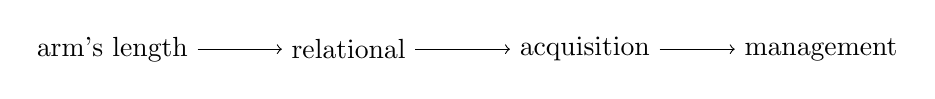
\begin{tikzpicture}
\node (a) at (0,0) {arm's length};
\node (b) at (3,0) {relational};
\node (c) at (6,0) {acquisition};
\node (d) at (9,0) {management};
\graph { (a) -> (b) -> (c) -> (d)};
\end{tikzpicture}




%% == Foreign owned firms perform better than domestic firms ==
%% * US: Doms and Jensen (1998)
%% * UK: Griffith (1999)
%% * Hungary, Romania, Russia, Ukraine: Brown, Earle, Telegdy (2006)
%% * Indonesia: Arnold and Javorcik (2009)
%% 
%% == Managers matter ==
%% * Good management practices  increase  productivity  (Bloom  and  Van  Reenen  2010;  Bloom  et  al.  2012;  Bloom  et  al.  2014) and market access (Bloom et al. 2016). 
%% * CEOs behaving like ``leaders" gradually improve firm performance. (Bandiera, Hansen, Prat and Sadun 2018)
%% * Large increase  in  the  level  and  inequality  of  CEO  pay.  (Murphy  and  Zábojník  2004;  Gabaix  and  Landier  2008;  Tervio  2008; Frydman and Saks 2010)
%% * Managers have persistent effects across firms on investment policy, R\&D, advertising, return on assets.  (Bertrand and Schoar 2003)
%% * Sudden CEO death worsens firm performance. (Bennedsen, Pérez-González and Wolfenzon 2007) 
%% * Managers having past export experience increase likelihood of exporting (Mion and Opromolla 2014; Mion, Opromolla and Sforza 2016) and importing (Bisztray, Koren and Szeidl 2018).




\end{frame}



\begin{frame}\frametitle{This paper}\hypertarget{This paper}{}
\begin{itemize}
\item Compile new data on which firm is run by which manager: Hungary, 1980--2018. 

\item Measure different degrees of foreign control:
\begin{enumerate}\setcounter{enumi}{0}
\item acquisition

\item replace CEO

\item hire expat CEO
\end{enumerate}

\item Results:
\begin{itemize}
\item Exporters and low-productivity firms become more tightly controlled. 

\item Firms with high immaterial capital receive local managers.

\item Foreign controlled firms become more productive and more likely to export. 




\end{itemize}

\end{itemize}
\end{frame}







\section{Data}\hypertarget{Data}{}


\begin{frame}\frametitle{Data}\hypertarget{Data}{}
\begin{block}{Hungarian Manager Database}\hypertarget{Hungarian Manager Database}{}
\begin{itemize}
\item coverage: universe of corporations, 1980--2018

\item CEO: highest officer of corporation as specified in corporate law.
\item information: name, mother's name, address, tenure at firm

\item 1 million firms, 2 million CEOs, 5 million job spells


\end{itemize}
\end{block}
\begin{block}{Balance sheet data}\hypertarget{Balance sheet data}{}
\begin{itemize}
\item coverage: universe of double entry firms, 1980--2018

\item information: sales, exports, employment, equipment, immaterials etc.


\end{itemize}
\end{block}
\end{frame}



\begin{frame}\frametitle{Names}\hypertarget{Names}{}
\begin{itemize}
\item We use manager names to infer 
\begin{enumerate}\setcounter{enumi}{0}
\item CEO change

\item nationality

\item gender (not used today)
\end{enumerate}

\item Foreign manager: firm representative with a non-Hungarian first name
\item e.g. Eva Bauer v Bauer Éva
\item but: George Soros v Soros György

\item Allow for misspelling, omitted middle name, missing data (jr, dr)


\end{itemize}
\end{frame}



\begin{frame}\frametitle{Sample}\hypertarget{Sample}{}
\item Exclude: 
\item employing less than 20 people
\item financial sector
\item domestic firms with expat CEO
\item greenfield FDI
\item firms with more than 15 CEOs
\item Left with 24,500 firms


\end{frame}







\section{Descriptives}\hypertarget{Descriptives}{}
\longfigure{input/ceo-panel/fig/manager-type-by-year/fig.pdf}{The number of CEOs increased sharply until 2010}
\longfigure{input/ceo-panel/fig/manager-type-by-age/fig.pdf}{The share of firms managed by founders gradually decreases with age}
\longfigure{input/ceo-panel/fig/tenure-by-type-weighted/fig.pdf}{Founders stay longest at the firm}








\section{Estimates}\hypertarget{Estimates}{}


\begin{frame}\frametitle{Degree of control}\hypertarget{Degree of control}{}
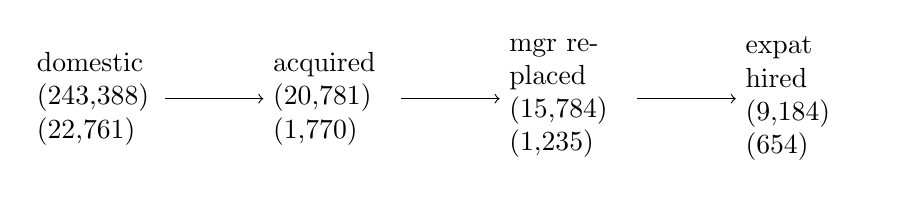
\begin{tikzpicture}
\node (a) [text width=1.5cm] at (0,0) {domestic (243,388) (22,761)};
\node (b) [text width=1.5cm] at (3,0) {acquired (20,781) (1,770)};
\node (c) [text width=1.5cm] at (6,0) {mgr replaced (15,784) (1,235)};
\node (d) [text width=1.5cm] at (9,0) {expat hired (9,184) (654)};
\graph { (a) -> (b) -> (c) -> (d)};
\end{tikzpicture}


\end{frame}



\begin{frame}\frametitle{Variables}\hypertarget{Variables}{}
\begin{itemize}
\item \alert{foreign}: firm has majority foreign owner

\item \alert{foreign\_hire}: firm has a manager hired by foreign owner

\item \alert{has\_expat}: firm has an expat manager

\item \alert{CONTROL${}^k$}: one of the three ($k=1,2,3$)

\item \alert{lnL}: log employment

\item \alert{lnQL}: log output per worker

\item \alert{TFP\_cd}: TFP (simple Cobb--Douglas)

\item \alert{exporter}: firm has positive exports

\item \alert{RperK}: share of immaterial assets in total [0,1]




\end{itemize}
\end{frame}



\begin{frame}\frametitle{Estimating equations}\hypertarget{Estimating equations}{}
\begin{block}{Bernard-Jensen}\hypertarget{Bernard-Jensen}{}
Sample: domestic firms and acquisitions
$$
Y_{ist} = \mu_{st} + \sum_{k=1}^3 \beta_k \text{CONTROL}_{it}^k + u_{ist}
$$


\end{block}
\begin{block}{Selection}\hypertarget{Selection}{}
Sample: $\text{CONTROL}_{i}^{k-1} = 1$, years before acquisition
$$
\text{CONTROL}_{i}^k = \mu_{st} + \gamma X_{it}  + u_{ist}
$$


\end{block}
\begin{block}{Diff-in-diff}\hypertarget{Diff-in-diff}{}
Sample: domestic firms and acquisitions
$$
Y_{ist} = \alpha_i + \mu_{st} + \sum_{k=1}^3 \beta_k \text{CONTROL}_{it}^k + u_{ist}
$$


\end{block}
\end{frame}



\begin{frame}\frametitle{Foreign firms are better in most respects}\hypertarget{Foreign firms are better in most respects}{}
\regressiontable{cross_section}


\end{frame}



\begin{frame}\frametitle{Positive selection on exports, negative on TFP}\hypertarget{Positive selection on exports, negative on TFP}{}
\regressiontable{selection}


\end{frame}



\begin{frame}\frametitle{Hiring an expat is associated with increased productivity and exporting}\hypertarget{Hiring an expat is associated with increased productivity and exporting}{}
\regressiontable{diffindiff}


\end{frame}



\begin{frame}\frametitle{Expats help start exporting, but have no effect on continuation}\hypertarget{Expats help start exporting, but have no effect on continuation}{}
\regressiontable{exporter}


\end{frame}







\section{Conclusions}\hypertarget{Conclusions}{}
\begin{frame}\frametitle{Conclusions}\hypertarget{Conclusions}{}
\begin{itemize}
\item What are the causes and consequences of foreign acquisitions?

\item We ask when managers are also replaced.

\item Using data on the universe of foreign acquisitions in Hungary, 1980-2018, we estimate that exporters and low-productivity firms become more tightly controlled. 

\item Foreign controlled firms become more productive and more likely to export. 

\item These facts help inform theories about the boundaries of global firms and about the role of managers in firm performance.


\end{itemize}
\end{frame}



\begin{frame}\frametitle{Next steps}\hypertarget{Next steps}{}
\begin{itemize}
\item Collect data on parent firms.

\item Build an incomplete-contract model.


\end{itemize}
\end{frame}







\end{document}